\documentclass{article}
\usepackage[margin=1in]{geometry}
\usepackage{amsmath}
\usepackage{xr}
\usepackage{xcolor}
\usepackage{siunitx}
\usepackage{gensymb}
\usepackage{graphicx}
\usepackage{wrapfig}
\usepackage{subcaption}

\externaldocument[S-]{Supporting_Information}
\externaldocument[M-]{Final_Draft}

\begin{document}

\graphicspath{{./figures/}}

\begin{center}
\textbf{Response to reviewers: Chemically Selective Transport in a Cross-linked 
H\textsubscript{II} Phase Lyotropic Liquid Crystal Membrane} \\
Authors: Benjamin J. Coscia and Michael R. Shirts
\end{center}

We thank the reviewers for carefully reading over our manuscript and providing
helpful comments. We have taken the suggestions into consideration and made
appropriate revisions to the manuscript document. All changes to the text have
been documented below. In cases where we modified the text we included the 
original text (denoted by ``Original text:") followed by the new text (denoted by
``New text:").

\section*{Response to Reviewer 1}

\begin{enumerate}
	
    \item \begin{quote} \textit{The manuscript, "Chemically Selective Transport 
    in a Cross-Linked H\textsubscript{II} Phase Lyotropic Liquid Crystal Membrane,"
    is an interesting effort that provides solid and never-before-developed insights
    into how structure and chemistry impact separations in an important new class of
    membrane materials. In particular, the ability to focus on and explain in a 
    rather complete manner that complex mechanisms that lead to results that are 
    below the Stokes-Einstein limit is impressive.  While somewhat verbose at times, 
    the manuscript is communicated in a clear manner, and it should be of interest 
    to a number of researchers in the field. As such, publication is recommended after
    the following minor points are addressed by the manuscript.} 
    \end{quote}
	
    Author reply: We thank the reviewer for their positive impression and feedback 
    and address their specific concerns below. 
	
    \item \begin{quote}
    \textit{The explanation regarding the transport of water molecules in the tail 
    region relative to water molecules in the pore region for the 5\% (by weight) 
    water system that occurs in the paragraph that begins at the end of page 20 is
    rather unsatisfying. While certain statistics are pointed to, there is not a 
    full explanation provided here. Expanding this point in order would strengthen
    the manuscript.}
    \end{quote}

    Author reply: We thank the reviewer for pushing us to strengthen our description
    of tail water transport in the 5 wt\% water system, as our point could be 
    confusing without proper explanation.

    %MRS: I'd leave out the text that stays the same (like the first sentence). 
    Original text: ``In the 5 wt\% water system, water molecules that spend the majority
    of their time in the distal tail region have MSDs slightly higher than those of water
    molecules close to the pore center. The MSD of distal tail water molecules is 1.7 nm$^2$
    compared to 1.2 nm$^2$ outside the distal tails. This anomaly is likely a consequence
    of lower density in the distal tails relative to the pores, leading to faster diffusion
    in the tails, as well as slowed diffusion of water molecules in the pores via hydrogen 
    bonds with other water molecules and association with sodium ions. Water molecules are 
    less likely to hydrogen bond with each other while in the distal tail region since they
    are interspersed between chains, while those in the pores stay in close proximity to 
    each other. We observed about 9 times more hydrogen bonding between water molecules 
    near the pore center versus those in the distal tail region. Additionally, an average 
    of 65\% of water molecules in the pores of the 5 wt\% water system are associated
    with a sodium ion each frame compared to 44\% in the 10 wt\% water system. There is a
    negligible amount of hydrogen bonds between water molecules and monomer head groups.
    
    New text: ``In the 5 wt\% water system, water molecules that spend the majority of their 
	time in the distal tail region have MSDs slightly higher than those of water molecules
	close to the pore center. The MSD of distal tail water molecules is 1.7 nm$^2$
	compared to 1.2 nm$^2$ outside the distal tails. The reason for this anomaly is twofold. 
	First, monomer head groups are concentrated about 0.2 nm closer to the pore centers
	in the 5 wt\% versus the 10 wt\% water system (see Figure~\ref{M-fig:component_densities})  %BJC: this is the RDF figure of head groups, tails, sodium, water
        %MRS: rather than saying there are more frequent collisions, I'd just say that it leaves less space, 
        %restricting the motion of the water.   
        which results in more frequent collisions between water molecules and relatively immobile 
	monomer head groups. 
        %MRS: but this next ``Second,'' doesn't explain why this slows things down more in 5%; just because the concentration of ions is higher?  But the concentration of water molecules is lower. 
        Second, the diffusion of water molecules is slowed via hydrogen
	bonds with other water molecules and association with sodium ions. Notably, there is a 
	negligible number of hydrogen bonds between water molecules and monomer head groups.
    The 95th percentile lifetime of hydrogen bonds between water molecules located near the
	pore center is 2.1 ns in the 5 wt\% system compared to 0.5 ns in the 10 wt\% system. 
	However, since we only saved simulation output every 0.5 ns, it is likely that the 
	true hydrogen bond lifetimes in the 10 wt\% system are smaller than this value. 
        %MRS: hmm the organization says: 2 effects, x and y.  Here is more about X. Here is more about Y. 
        %MRS to make clear what is being talked about where, it might be better to say: ``There are 2 effects. Here is X, here is Y.''
        %MRS: don't start with dependent clauses.  This logic makes sense, but the above one doesn't so much, 
        %MRS: because it's not made clear why the H-bonds are lasting longer (clearly, if they are lasting longer, MSD will go up). 
	With regard to sodium ions, more frequent and longer periods of association
	with water molecules helps to drive down water's MSD. An average of 65\% of water 
	molecules in the pores of the 5 wt\% water system associate with a sodium ion each
	frame compared to 44\% in the 10 wt\% water system. There are about half as many water
	molecules in the 5 wt\% water system which allows a larger fraction of them to associate
	with sodium ions. The lifetime of associations between sodium ions and water is 7.5 ns
	and 3.0 ns in 5 and 10 wt\% water systems respectively.  ``
	
    \item \begin{quote}
    \textit{The final paragraph of the conclusions of the manuscript ends on a blunt, and 
    somewhat pessimistic, note. That is, there is no doubt that there are complicated 
    interactions that will occur in many membrane separations, and that it is not always 
    easy to predict beforehand what the results will be. However, the strategy outlined 
    by this effort provides at least a footing by which to attack certain problems. This
    work provides atomistic modeling that does more than just allow one to think critically
    about nanostructured membranes. In fact, one might argue that one does not necessarily
    need such complex computational powers to think critically about nanostructured 
    membranes. Instead, one might argue that these kinds of efforts provide insights that
    would not necessarily be obvious from simple "chemical intuition" points of view that 
    are typically relied upon by many membrane scientists. As such, it might be useful to
    highlight where this effort provided insights that were not necessarily obvious as the
    end of the manuscript. This might serve as a means by which to entice experimentalist
    to incorporate these kinds of efforts into their own work such that the pace at which
    discoveries are made by the entire community is increased.}
    \end{quote}
	
    Author reply: We thank the reviewer for encouraging us to strengthen our conclusions and
    to end on a more positive note. We have modified our final paragraph with this in mind 
    and to emphasize that these types of studies are 
    %necessary to identify
    very valuable in identifying
    transport behavior
    that might not be obvious based solely on intuition
    %MRS: added
    or bulk scale experiments.
    
    Original text: ``The findings here are likely too complex to point towards a clear 
    design of an optimal LLC membrane for a particular separation. This work does demonstrate
    that there is a large range of solute-membrane interactions resulting from the
    chemically complex and inhomogeneous LLC membrane structure. The varying chemical 
    functionality of the solutes themselves gives rise to an immense diversity of transport 
    behavior. This behavior suggests that a large range of chemical selectivities may be 
    possible in self-assembled nanoporous membranes. Atomistic modeling gives us the 
    opportunity to observe these interactions at the molecular scale, at least approximately,
    so that we can think more critically about nanostructured membrane design.''
    
    New text: ``Our work demonstrates that one cannot rely solely on chemical intuition while 
    designing LLC membranes for particular separations. 
    %MRS5: Hmm.  Still not quite: we want to communicate ``experiment PLUS
    %simulations!'' not ``experiments are not enough''. How about something more like this?
    %``Our work demonstrates that there are important, atomistic features of nanostructed, self-assembled materials 
    % that molecular simulation can play a key role in elucidating''
    The complex interplay between the
    inhomogeneous membrane structure, solute size and solute functionality leads to a variety of
    solute-membrane interactions, of which many are quite subtle. For example, association
    between polar groups and ions is seldom mentioned in the literature, but we could not give a
    complete mechanistic explanation of observed transport behavior without its consideration. 
    %MRS: is there a second example you can put in as well?
    The interactions we observed, along with those that may arise in 
    %MRS: simpler
    %alternative 
    other
    self-assembled
    nanoporous membranes, 
    %can lead to an substantial
    have the potential to produce an immense 
    diversity of transport behavior, 
    %which suggests
    suggesting
    that a 
    %MRS: 
    previously unexplored range
    %large range 
    of chemical selectivities may be possible. Atomistic molecular modeling
    %MRS: maybe a bit overkill
    %may be the best hope of
    is likely to be highly useful in
    uncovering 
    %the dominant 
    important 
    mechanisms that will inspire and accelerate
    novel design by experimentalists.''
	
\end{enumerate}

\section*{Response to Reviewer 2}

\begin{enumerate}
	
	\item \begin{quote} \textit{Using all-atom classical molecular dynamics (MD) simulations,
	the authors examined the transport properties of water, sodium ions and a total of 20 
	small polar solutes in a model lyotropic liquid crystal (LLC) membrane, specifically the
	hexagonal HII phase formed by the liquid crystal monomer Na-GA3C11. This is a very 
	detailed and brilliantly done molecular simulation study, where the data was carefully 
	analyzed to provide molecular-level insights about these systems that will be very 
	useful to experimentalists working with this type of membrane for water purification 
	purposes. I only have the following minor comments: }\end{quote}
	
	Author reply: We thank the reviewer for the kind assessment of our work. We address their
	comments below.
	
	\item \begin{quote}
	
	\textit{The water model used by the authors was not explicitly mentioned in Section 2 
	of the paper. From the Results section it is inferred that they used the TIP3P water model.
	The authors should explicitly mention their choice of water model in Section 2, and 
	justify this choice.}
	
	\end{quote}
	
	Author reply: We thank the reviewer for pointing out that we are missing this essential detail.
	We have added the following text to section 2.1 of the main text:

	New text: ``We simulated water molecules using the TIP3P water model because it is 
    computationally efficient and reasonably reproduces water's physical properties
    at 300K, the temperature of our simulations.``
        %MRS3: TIP-4P is pretty close in efficiency, and TIP3P is only mediocre in bulk water properties  I would probably say that TIP3P was used because it is the water model that GAFF and other AMBER family parameters were optmized with.  TIP3P also diffuses faster than experimental water, which is both a negative (can't compare absolute diffusion) and positive (things happen faster). 
  	We also added the following citation in support of our justification:
  	
        %MRS: that's the TIP5P paper, though . . . did you mean to cite it?
  	Mahoney, M. W.; Jorgensen, W. L. A Five-Site Model for Liquid Water and the Reproduction
  	of the Density Anomaly by Rigid, Nonpolarizable Potential Functions. J. Chem. Phys. 2000, 
  	112, 8910–8922
    
    \item \begin{quote}
    
    \textit{The Methods section should contain more details about the model membranes, for 
    example the length of the pores in the z-direction, the range of pore sizes (I understand
    they vary with water content), and the range of distances between the center of adjacent pores.}    
    
    \end{quote}
    
    Author reply: We thank the reviewer for this suggestion. We agree that it would be useful
    to our readers if we included more details about our models. We have added the following 
    text to Section 2.2 of our Methods.
    
    %BJC: not sure what else to include.  Don't want to say anything about pore size
    %BJC: density is about the same 
    New text: ``The equilibrated unit cells have different geometries depending on water content. 
    The average distance between pores is 4.15 +/- 0.08 nm and 4.41 +/- 0.07 nm
    in the 5 and 10 wt\% water systems respectively. The length of the pores, accounting
    for tortuosity (see Section~\ref{M-method:rdfs}), is 9.03 +/- 0.12 nm and 8.07 +/- 0.11
    nm in the 5 and 10 wt\% water systems respectively.''  
    % BJC: not sure what if anything to say about difference in lengths of pores (which is roughly
    % equivalent to the box dimension in the z-direction). My guess is that when monomers don't 
    % stack directly on top of each other, they can pack tighter in the z-direction. When there
    % is more water, they are more disordered and can move away or closer to the pore center which
    % facilitates that packing. The RDF of head groups in the 10 wt% versus 5 wt% is broader (density
    % at peak is lower) which supports this. But that kind of discussion isn't suitable for methods,
    % and I don't think it's really in the scope of the paper. Would just add more words.

    %MRS: I would actually put this argument more clearly in the paper
    %- if the reviewer missed it, readers will as well.  If it's in
    %there already, I would emphasize it, and then mention here where
    %it was added, and cite the previous paper - it was one of the main messages of that paper.
    We elected to not include pore sizes because its definition is ambiguous. There is not a 
    hard partition between the pore and tails. Rather, there is a gradual transition from 
    the hydrophilic to hydrophobic region. 
    The approximate size of the pore region and the 
    boundaries we defined are addressed later in the methods and throughout the results and 
    discussion section.
    
    \item \begin{quote}
    
    \textit{I think most of the text related to preparation of the model systems (Section S2, 
    Supporting Information), should be moved into the Methods section of the paper. I believe 
    these simulation setup details are important to researchers working with somewhat similar 
    systems.}
    
    \end{quote}
    
    Author reply: We thank the reviewer for their suggestion. We've edited Section 2.2 of the main
    text to include a consolidated discussion of the data and analysis presented in Section S2, 
    while leaving the full discussion in Section S2.
    
    Old text: `` We observed that some water partitions into the distal tail region of our system and therefore
	built our initial configurations with water in both regions, close to the expected
	equilibrium partition (see Section~\ref{S-section:water_content_equil} of the Supporting
	Information). We define the distal tail region to be ca. 1.5 nm from the pore
	center based on the minimum in the radial distribution function of water
	(see Section~\ref{M-method:rdfs}). The amount of water present in the distal tail region
	may or may not be experimentally consistent but it is necessary for our results to be 
	thermodynamically consistent; otherwise, water would slowly leak from the pore into the
	tail region over several hundred nanoseconds. We iteratively adjusted the pore radius in our systems
	until the appropriate amount of water fit in the pores after running the GROMACS command
	\texttt{gmx solvate}. We placed water molecules in the distal tail region one at a time
	in random locations with a short energy minimization between each insertion. When 
	studying transport of water in the pores, we limited the calculations to water molecules
	that spent greater than 95\% of their time outside of the distal tail region. We 
	justify this decision with better context in Section~\ref{M-section:transport_water_sodium}.
	
    First, we equilibrated the initial configuration using the `wet' equilibration procedure 
	described in our previous work. Then we cross-linked the equilibrated solvated 
	configuration using the cross-linking procedure also described in our previous 
    work.''
           
    New text: `` We initially attempted to equilibrate our system with water by allowing water
	molecules to naturally penetrate the membrane from a water bath separating
	periodic images of the system in the $z$-direction. We allowed a dry, previously
	equilibrated system to further equilibrate in coexistence with a 3 nm-thick 
	(in the $z$-direction) layer of water. Although the water appears to equilibrate
	after 1000 ns of simulation, the density of water along the pore axis
	is close to zero at the membrane center, implying that there is a kinetic
	barrier to water filling the pores which we will be unable to overcome using
	conventional simulations. See Section~\ref{S-section:water_content_equil} 
        %MRS: will need to get the references working using xr or manually for the letter.
        of the Supporting Information for an expanded explanation and supporting figures. 
	  
        %MRS: might want to make it clear that this below is a separate feature, observed in 
        %different simulations than the ones above.
	We observed water enters into the distal tail region of our system. We define the 
	distal tail region to be ca. 1.5 nm from the pore center based on the minimum in 
	the radial distribution function of water (see Section~\ref{M-method:rdfs}). Therefore
	we aimed to build our initial configurations with water in both regions, close to
	the expected equilibrium partition. The final amount of water present in the distal
	tail region may or may not be experimentally consistent but it is necessary for our
	results to be thermodynamically consistent; otherwise, water would slowly leak 
	from the pore into the tail region over several hundred nanoseconds. 
	
	To determine the approximate ratio of water in the pores to tails, we equilibrated 4 systems
	where we initially placed water in the pores and in the tails in addition to a water
	reservoir between periodic images. We filled the pores with water by running the 
	GROMACS command \texttt{gmx solvate} on our initial configuration followed by the 
	removal of any water molecules placed in the distal tail region. This method requires
	that we vary the 
        %MRS: is ``initial pore radius'' a good phrase to use, since we are fighting against the idea of 
        % well-defined pore radii?  ``monomer starting radius?''
        initial pore radius since the vacant space dictates the pore's 
	water content. We then placed a defined number of water molecules into the distal tail
	region one at a time with a short energy minimization between each insertion.
	We chose to test systems with initial pore radii of 5, 6, 7 and 8 \AA~with tail and 
	pore water compositions given in Table~\ref{table:water_content}. We found that 
	systems started with more water in the pores than tails tended to equilibrate relatively
	quickly with an approximate ratio of 3 water molecules in the pores to 2 in the tails.

    % BJC: could go back in supporting
    % MRS: I could go either way.
    \begin{table}[!htb]
    \centering
    \begin{tabular}{|c|c|c|}
    \hline
    Pore Radius (\AA) & wt \% water tails & wt \% water pores \\
    \hline
    5                 &        5.67       &     1.09          \\
    6                 &        2.88       &     2.38          \\
    7                 &        1.91       &     4.12          \\
    8                 &        2.78       &     6.00          \\
    \hline
    \end{tabular}
    \caption{We chose a diverse combination of initial pore and tail water
    contents in order to study its effect on equilibrium water
    content.}\label{table:water_content}
    \end{table}

    %MRS: is this figure below moving to the front?  I think may be it still is more of a supporting figure.
    \begin{figure}[!htb]
    \centering
    \begin{subfigure}{0.45\textwidth}
    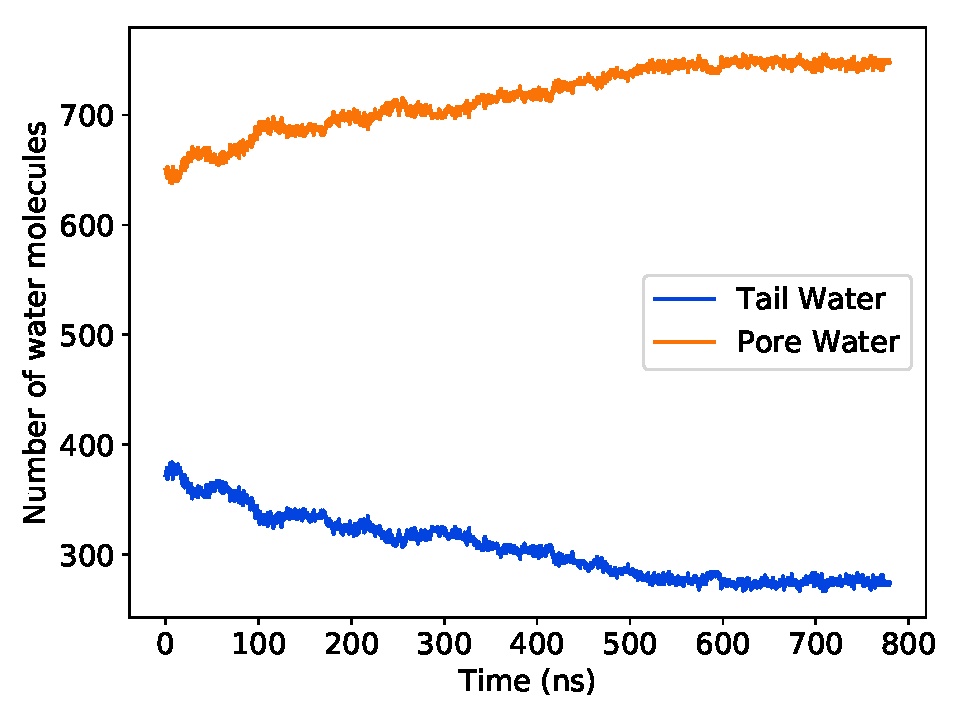
\includegraphics[width=\textwidth]{5wt_offset_equil.pdf}
    \caption{5 wt \%}\label{fig:5wt_offset_equil}
    \end{subfigure}
    \begin{subfigure}{0.45\textwidth}
    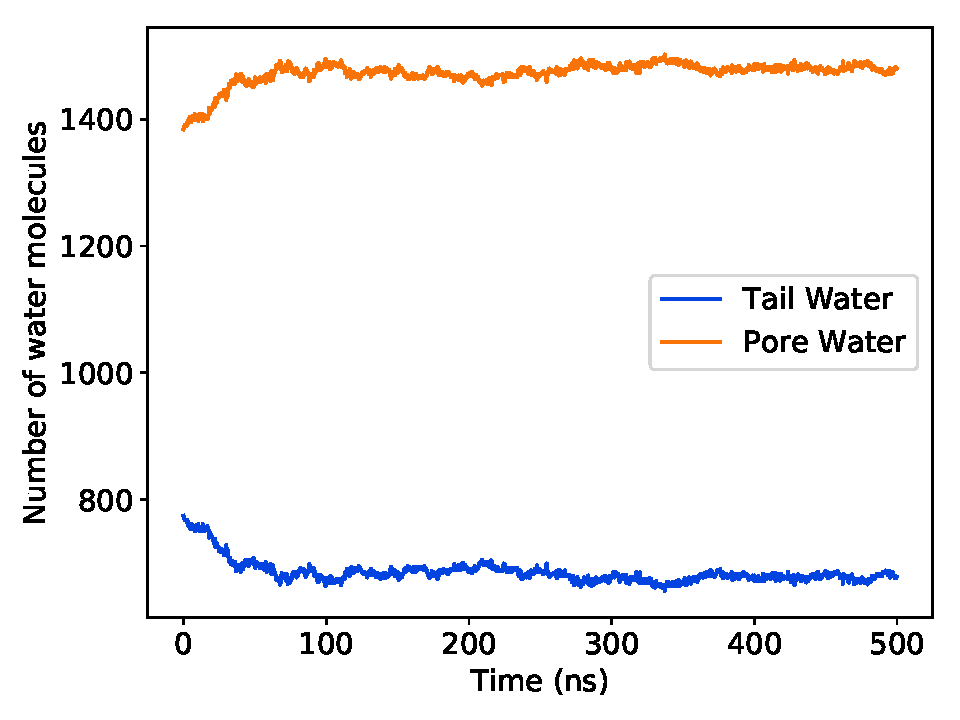
\includegraphics[width=\textwidth]{10wt_offset_equil.pdf}
    \caption{10 wt \%}\label{fig:10wt_offset_equil}
    \end{subfigure}
    \caption{We created solvated systems with one third of the total water
	  initially placed in the tail region. (a) With 5 wt \% total water, the water
	  content equilibrates after 600 ns, with $\sim$ 72 \% of the total water in the
	  pores. (b) With 10 wt \% total water, the water content equilibrates after 100
	  ns, with $\sim$ 69 \% of the total water in the
	  pores.}\label{fig:solvation_equilibration}
    \end{figure}
  
    We removed the water reservoir and allowed the pore and tail water
    contents to equilibrate with 5 and 10 wt\% total water with a 3:2 ratio
    of pore to tail water. We considered the water content
    equilibrated once the water contents plateaued. The 5 wt\% system did
    not plateau until $\sim$ 600 ns (Figure~\ref{fig:5wt_offset_equil})
    while the 10 wt \% water system equilibrated within the first 100 ns of 
    simulation (Figure~\ref{fig:10wt_offset_equil}).
    The equilibrated pores contain 72 \% and 69 \% of the total water in the
    5 and 10 wt \% systems respectively. We cross-linked the equilibrated 
    solvated systems, then allowed them to equilibrate further for 100 ns. 
    The water contents in each region does not change significantly in either case 
    (see Figure~\ref{S-fig:xlinked_solvation_equilibration} of the Supporting Information).
    The `wet' equilibration and cross-linking procedures follow
    the methods outlined in our previous work.''

\end{enumerate}

\end{document}
